\documentclass{standalone}
\usepackage{bm}
\usepackage{tikz}
\usetikzlibrary{arrows,decorations.pathreplacing, decorations.shapes,external}
\tikzexternalize

\newcommand\spiral{}% Just for safety so \def won't overwrite something
\def\spiral[#1](#2)(#3:#4:#5){% \spiral[draw options](placement)(end angle:revolutions:final radius)
\pgfmathsetmacro{\domain}{pi*#3/180+#4*2*pi}
\draw [#1,
       shift={(#2)},
       domain=0:\domain,
       variable=\t,
       smooth,
       samples=int(\domain/0.08)] plot ({\t r}: {#5*\t/\domain})
}

\begin{document}

% turning points
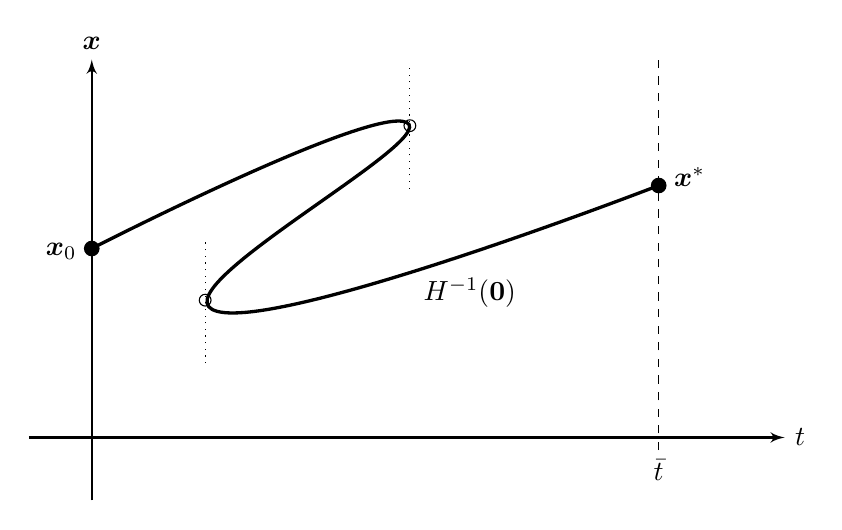
\begin{tikzpicture}[
		p1/.style={circle,fill,inner sep=2pt},
		p2/.style={circle,draw,inner sep=1.5pt},
		>=latex',
		scale=0.8]
	%% axis
	\draw[thick,->] (-1,0) -- (11,0) node[right] {$t$};
	\draw[thick,->] (0,-1) -- (0,6) node[above] {$\boldsymbol{x}$};
	\draw[dashed] (9,-0.2) node[below] {$\bar{t}$} -- (9,6);
	%% define path
	\draw[very thick] plot [smooth, tension=1] coordinates {(0,3) (5,5) (2,2) (9,4)};
	%% define beginning and end
	\node at (0,3) [p1, label={[left,xshift=-2pt,yshift=-4pt] $\boldsymbol{x}_0$}] {};
	\node at (9,4) [p1, label={[right,xshift=2pt,yshift=0pt] $\boldsymbol{x}^*$}] {};
	\node at (6,2.3) {$H^{-1}(\boldsymbol{0})$};
	%% define turning points
	\node at (5.05,4.95) [p2] {};
	\draw[dotted] (5.05,3.95) -- (5.05,5.95);
	\node at (1.8,2.18) [p2] {};
	\draw[dotted] (1.8,1.18) -- (1.8,3.18);
\end{tikzpicture}

% shapes of path: tracing infeasible
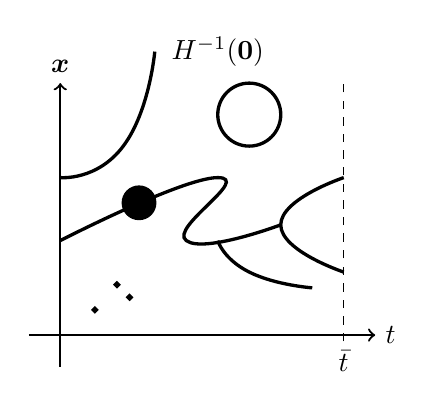
\begin{tikzpicture}[scale=0.4]
	%% axis
	\draw[thick,->] (-1,0) -- (10,0) node[right] {$t$};
	\draw[thick,->] (0,-1) -- (0,8) node[above] {$\boldsymbol{x}$};
	\draw[dashed] (9,-0.2) node[below] {$\bar{t}$} -- (9,8);
	%% define path
	\node at (5,9) {$H^{-1}(\boldsymbol{0})$};
	\draw[very thick] plot [smooth, tension=1] coordinates {(0,3) (5,5) (4,3) (7,3.5)};
	\draw[very thick] plot [smooth, tension=1] coordinates {(9,5) (7,3.5) (9,2)};
	\draw[very thick] plot (6,7) circle[radius=1];
	\filldraw[very thick] plot (1.1,0.8) circle[radius=0.05];
	\filldraw[very thick] plot (1.8,1.6) circle[radius=0.05];
	\filldraw[very thick] plot (2.2,1.2) circle[radius=0.05];
	\draw[very thick] plot [smooth, tension=1] coordinates {(5,3) (6,2) (8,1.5)};
	\spiral[very thick](5.3,1.3)(45:4:1);
	\draw[very thick] plot [smooth, tension=1] coordinates {(0,5) (2,6) (3,9)};
	\filldraw[very thick] plot (2.5,4.2) circle[radius=0.5];
\end{tikzpicture}
% shapes of path: tracing feasible
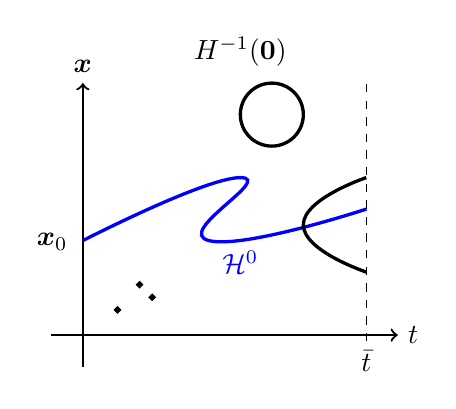
\begin{tikzpicture}[scale=0.4]
	%% axis
	\draw[thick,->] (-1,0) -- (10,0) node[right] {$t$};
	\draw[thick,->] (0,-1) -- (0,8) node[above] {$\boldsymbol{x}$};
	\draw[dashed] (9,-0.2) node[below] {$\bar{t}$} -- (9,8);
	%% define path
	\node at (5,9) {$H^{-1}(\boldsymbol{0})$};
	\node[blue] at (5,2.3) {$\mathcal{H}^0$};
	\draw[very thick, blue] plot [smooth, tension=1] coordinates {(0,3) (5,5) (4,3) (9,4)};
	\node at (0,3) [label={[left,xshift=-2pt,yshift=-4pt] $\boldsymbol{x}_0$}] {};
	\draw[very thick] plot [smooth, tension=1] coordinates {(9,5) (7,3.5) (9,2)};
	\draw[very thick] plot (6,7) circle[radius=1];
	\filldraw[very thick] plot (1.1,0.8) circle[radius=0.05];
	\filldraw[very thick] plot (1.8,1.6) circle[radius=0.05];
	\filldraw[very thick] plot (2.2,1.2) circle[radius=0.05];
\end{tikzpicture}

% predictor-corrector procedure
\begin{tikzpicture}[
		p1/.style={circle,fill,inner sep=2pt}, 
		p2/.style={circle,draw,inner sep=1.5pt},
		p3/.style={circle,draw,inner sep=1pt},
		>=latex']
	%% define path
	\draw[very thick] plot [smooth, tension=1] coordinates {(0,0) (4,5) (10,2)};
	\node[below] at (10,2) {$H(\boldsymbol{y})=\boldsymbol{0}$};
	%% define points
	\node (yi) at (0.78,2) [p1, label={[below right,xshift=2pt] $\boldsymbol{y}_k$}] {};
	\node (yi0) at (4,8) [p2, label={[above left,xshift=2pt,yshift=-2pt] $\boldsymbol{y}_k^0$}] {};
	\node (yi0x) at (4.7,8.7) {};
	%(5,7.5)
	\node (yi1) at (5,7) [p3, label={[below left,xshift=-2pt,yshift=4pt] \footnotesize $\boldsymbol{y}_k^1$}] {};
	\node (yi1x) at (5.85,7.5) {};
	\node (yi2) at (5.4,6.2) [p3, label={[left,xshift=-2pt,yshift=-2pt] \footnotesize $\boldsymbol{y}_k^2$}] {};
	\node (yi2x) at (6.3,6.4) {};
	\node (yi3) at (5.5,5.8) [p3, label={[left,xshift=-2pt,yshift=-4pt] \footnotesize $\boldsymbol{y}_k^3$}] {};
	\node (yi3x) at (6.4,5.8) {};
	\node (yi4) at (5.5,5.3) {};
	\node (yin) at (5.4,5.3) {};
	\node (yj) at (5.3,5) [p1, label={[below,xshift=-4pt,yshift=-6pt] $\boldsymbol{y}_{k+1}$}] {};
	\node (yj0) at (9,4.1) [p2, label={[right,yshift=-2pt] $\boldsymbol{y}_{k+1}^0$}] {};
	%% define arrows
	\draw[->,thick] (yi) -- (yi0);
	\draw[decoration={brace,amplitude=10pt,raise=30pt},decorate] (yi) -- (yi0) node[midway,above left,xshift=-32pt,yshift=15pt] {\footnotesize $ds$};
	\draw[->] (yi0) -- (yi0x);
	\draw[->,thick,dotted] (yi0) -- (yi1);
	\draw[->] (yi1) -- (yi1x);
	\draw[->,thick,dotted] (yi1) -- (yi2);
	\draw[->] (yi2) -- (yi2x);
	\draw[->,thick,dotted] (yi2) -- (yi3);
	\draw[->] (yi3) -- (yi3x);
	\draw[->,thick,dotted] (yi3) -- (yi4);
	\draw[->,thick,dotted] (yin) -- (yj);
	\draw[->,thick] (yj) -- (yj0);
\end{tikzpicture}

%  simple bifurcation
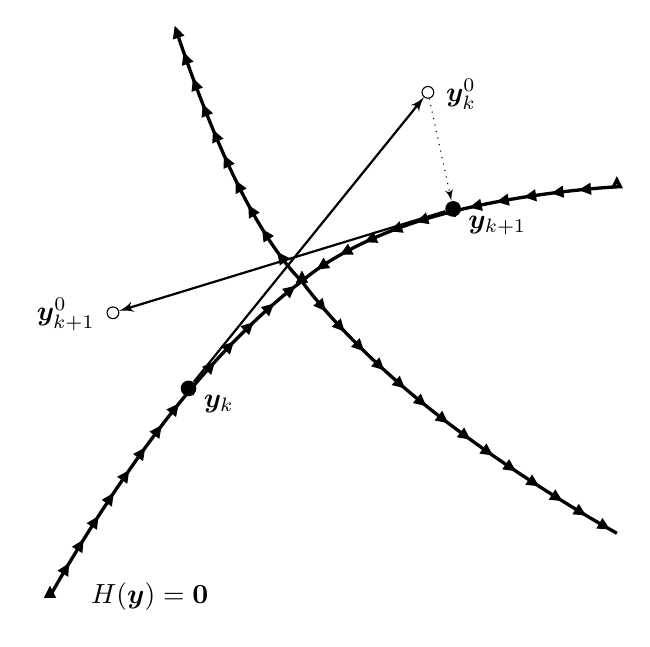
\begin{tikzpicture}[
		p1/.style={circle,fill,inner sep=2pt}, 
		p2/.style={circle,draw,inner sep=1.5pt},
		>=latex',
		scale=0.8]
	%% define path
	\draw[very thick,decoration=triangles,postaction={draw,decorate}] plot [smooth, tension=1] coordinates {(0,0) (2,3) (4,5)};
	\draw[very thick,decoration=triangles,postaction={draw,decorate}] plot [smooth, tension=1] coordinates {(9,6.5) (6,6) (4,5)};
	\draw[very thick,decoration=triangles,postaction={draw,decorate}] plot [smooth, tension=1] coordinates {(4,5) (3,6.5) (2,9)};
	\draw[very thick,decoration=triangles,postaction={draw,decorate}] plot [smooth, tension=1] coordinates {(4,5) (6,3) (9,1)};
	\node[right] at (0.5,0) {$H(\boldsymbol{y})=\boldsymbol{0}$};
	%\draw[->] (9,3) node[right] {$det\begin{pmatrix}J(\boldsymbol{y})\\t(\boldsymbol{y})\end{pmatrix}=\boldsymbol{0}$} to[out=180,in=0] +(-4.8,+2);
	%% define points
	\node (yi) at (2.2,3.3) [p1, label={[below right,xshift=2pt,yshift=-2pt] $\boldsymbol{y}_k$}] {};
	\node (yi0) at (6,8) [p2, label={[right,xshift=3pt,yshift=-3pt] $\boldsymbol{y}_k^0$}] {};
	\node (yj) at (6.4,6.15) [p1, label={[below right,xshift=2pt,yshift=-2pt] $\boldsymbol{y}_{k+1}$}] {};
	\node (yj0) at (1,4.5) [p2, label={[left,xshift=-3pt,yshift=-3pt] $\boldsymbol{y}_{k+1}^0$}] {};
	%% define arrows
	\draw[->,thick] (yi) -- (yi0);
	\draw[->,dotted] (yi0) -- (yj);
	\draw[->,thick] (yj) -- (yj0);
\end{tikzpicture}

% path jumping
\begin{tikzpicture}[
		p1/.style={circle,fill,inner sep=2pt}, 
		p2/.style={circle,draw,inner sep=1.5pt},
		>=latex',
		scale=0.8]
	%% define path
	\draw[very thick] plot [smooth, tension=1] coordinates {(0,0) (4,3) (10,3)};
	\draw[very thick] plot [smooth, tension=1] coordinates {(2,9) (4,6) (10,6)};
	\node[above] at (10,4) {$H(\boldsymbol{y})=\boldsymbol{0}$};
	%% define points
	\node (yi) at (2,2.1) [p1, label={[below right,xshift=2pt,yshift=-2pt] $\boldsymbol{y}_k$}] {};
	\node (yi0) at (5,4.6) [p2, label={[right,xshift=3pt,yshift=-3pt] $\boldsymbol{y}_k^0$}] {};
	\node (yj) at (5.1,5.7) [p1, label={[above,xshift=2pt,yshift=2pt] $\boldsymbol{y}_{k+1}$}] {};
	%% define arrows
	\draw[->,thick] (yi) -- (yi0);
	\draw[->,dotted] (yi0) -- (yj);
\end{tikzpicture}

\end{document} 
